\subsection{Diagramme de classes}
\begin{frame}{Diagramme de classes}
\begin{figure}
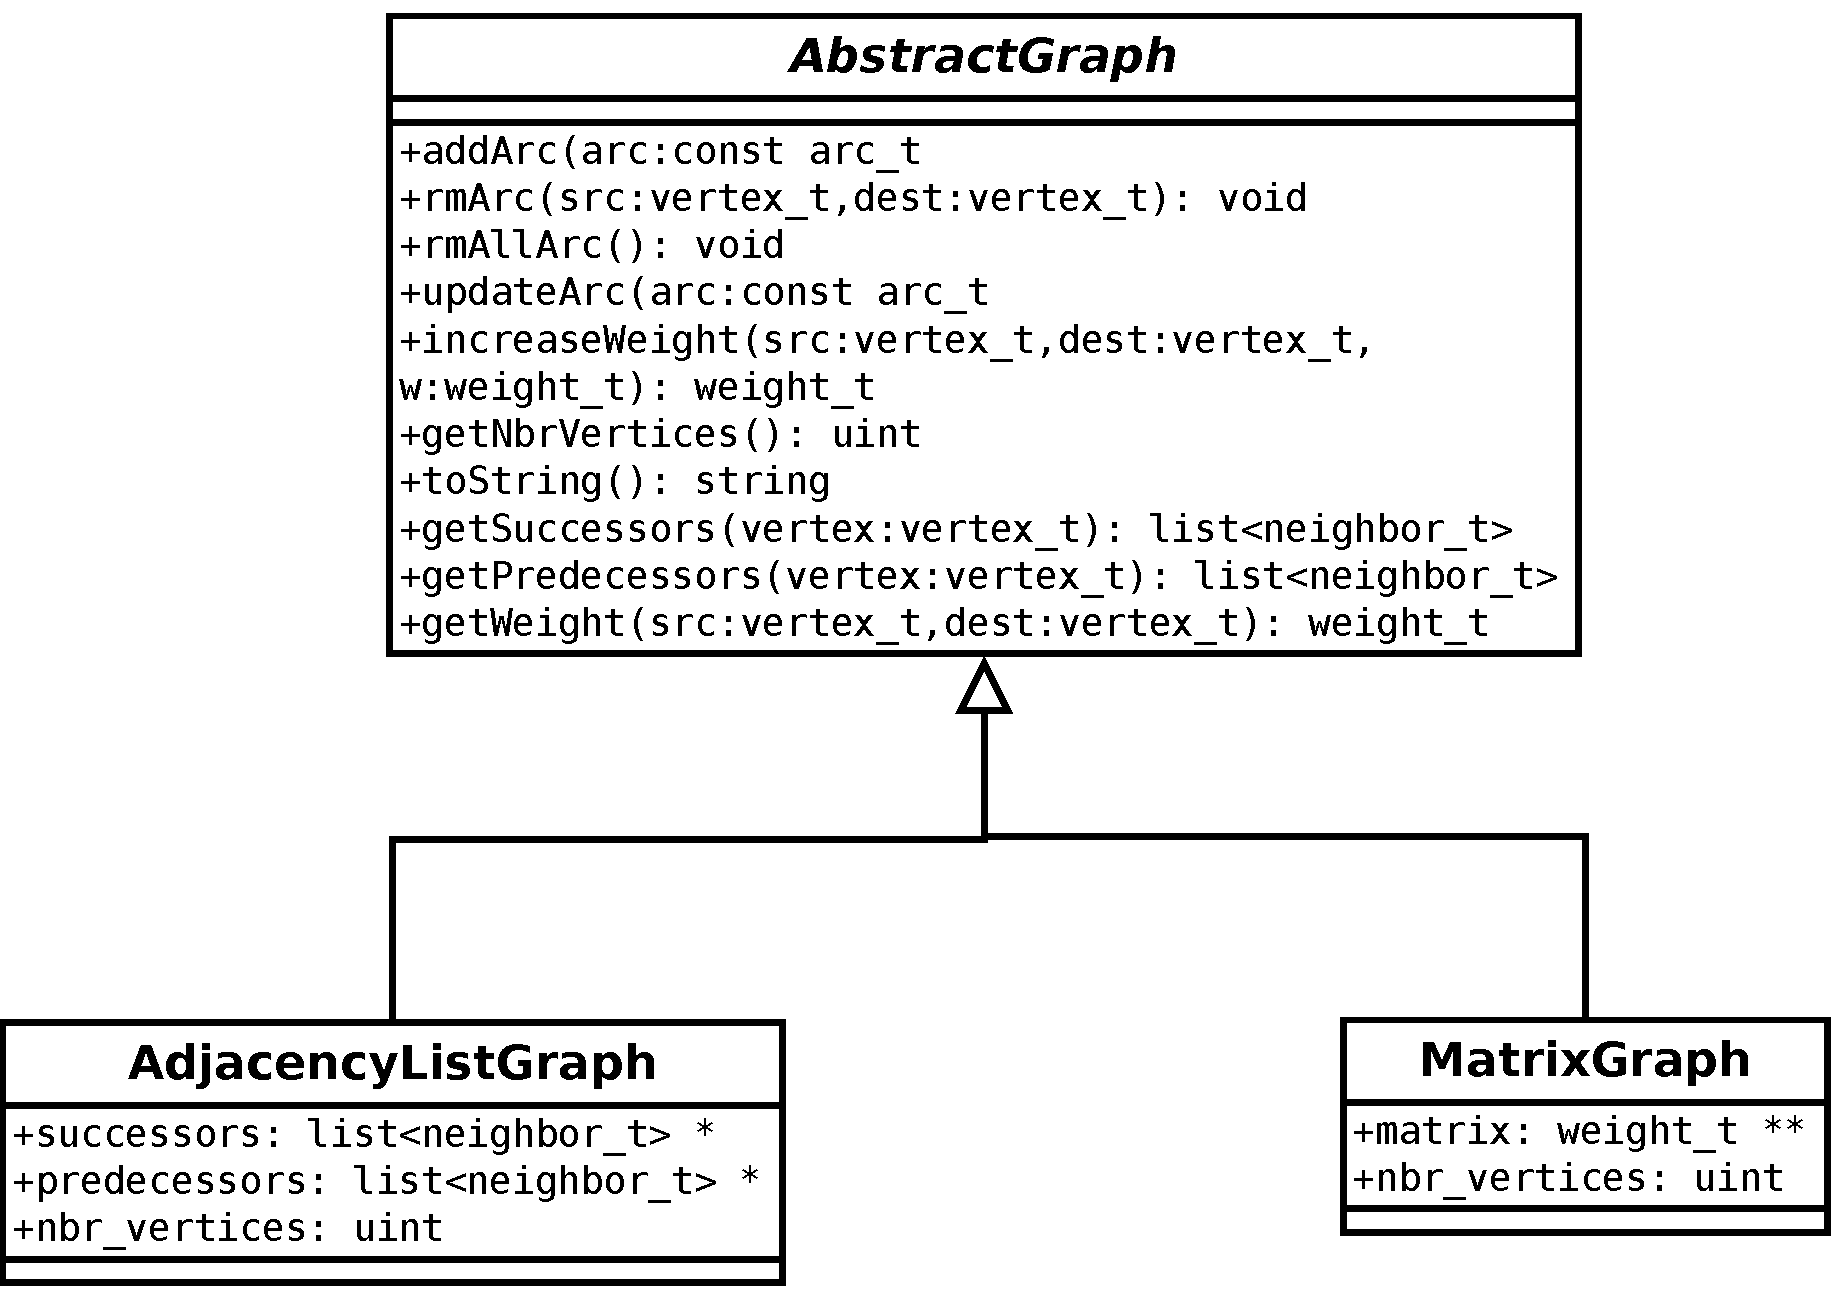
\includegraphics[width=0.8\textwidth]{img/diag_class.pdf}
\end{figure}
% Classe abstraite pour s'abstraire dans les algos des structures de données
% ...
\end{frame}

\subsection{Génération de réseaux de transport aléatoires}
\begin{frame}{Génération de réseaux de transport aléatoires}
\begin{block}{Stratégie de génération}
  \begin{itemize}
    \item génération de n points
    \item génération d'un chemin de taille n
  \end{itemize}
\end{block}
\end{frame}

\subsection{Choix techniques}
\begin{frame}{Choix techniques}
\begin{itemize}
\item Choix du langage
\item Choix d'implémentation
\item Etc\ldots
\end{itemize}
\end{frame}


\begin{frame}{Choix techniques}{Structures de données}
\end{frame}

\subsection{Fonctionnement général}
\begin{frame}{Fonctionnement général}
\end{frame}